\documentclass{beamer}
\usetheme{dianahep}

%
% Title definitions
%

\title{Conceptualization of an NSF Scientific Software Innovation Institute for High Energy Physics (S2I2-HEP)}
\author{Peter Elmer - Princeton University \\
        Mark Neubauer - University of Illinois at Urbana-Champaign \\
        Mike Sokoloff - University of Cincinnati \\  
        \url{http://s2i2-hep.org}}
\date{10 April, 2018 \\ URSSI Kick-off Workshop}

\begin{document}
\maketitle
%\insertframenumber/\inserttotalframenumber

%
% Presentation body
%

\setbeamertemplate{footline}[frame number]

% S2I2 HEP introdution

\begin{frame}
\frametitle{S2I2-HEP Conceptualization - http://s2i2-hep.org}

\begin{figure}[t]
\begin{center}
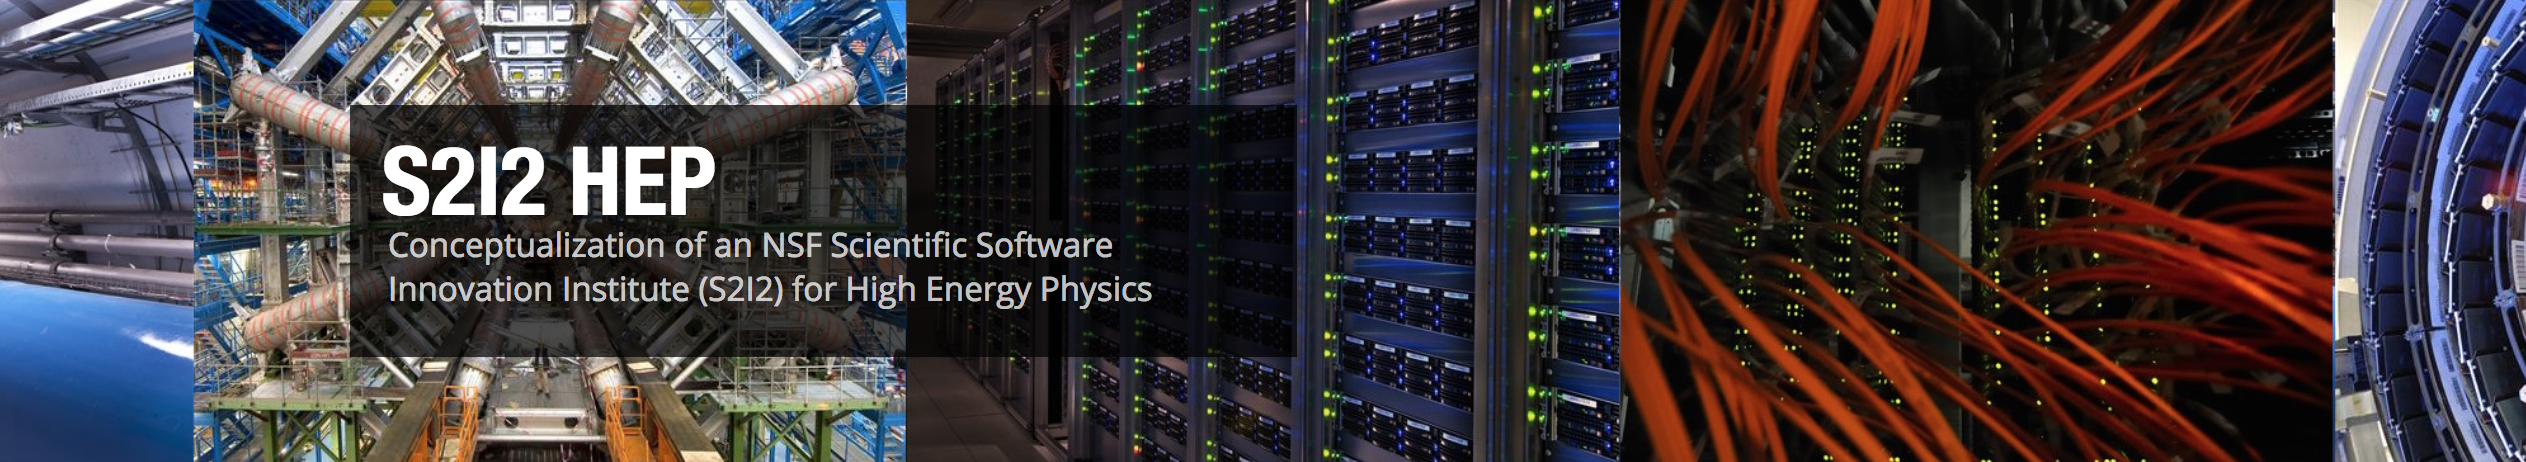
\includegraphics[width=0.9\textwidth]{images/s2i2-hep-website-banner.png}
%\caption{}
%\label{fig:example2}
\end{center}
\end{figure}

\small{The primary goal of the S2I2-HEP conceptualization project is to prepare a strategic plan for a potential NSF Scientific Software Innovation Institute (S2I2) to develop software for experiments taking data in the ``High-Luminosity Large Hadron Collider'' (HL-LHC) era in the 2020s.}
\vskip 0.1in
\small{S2I2-HEP sponsors community workshops and conceptual work to ``take advantage of the significant data and computing requirements of the Large Hadron Collider as a science driver for next generation high-performance software and sustainability developments.''}
\end{frame}



\begin{frame}
\frametitle{HEP Science Drivers - Beyond the ``Standard Model''}

The {\em Strategic Plan for U.S.\ Particle Physics} from May, 2014 (the
last community ``decadal survey'' and planning exercise for US HEP)
identified ``five compelling lines of inquiry that show 
great promise for discovery over the next 10 to 20 years.''
These are the Science Drivers:
\begin{itemize}
 \item Use the Higgs boson as a new tool for discovery
 \item Pursue the physics associated with neutrino mass
 \item Identify the new physics of dark matter
 \item Understand cosmic acceleration: dark matter and inflation
 \item Explore the unknown: new particles, interactions, and physical principles.
\end{itemize}

\end{frame}



\begin{frame}
\frametitle{Large Hadron Collider (LHC) and Experiments}

\begin{figure}[htbp]
\begin{center}
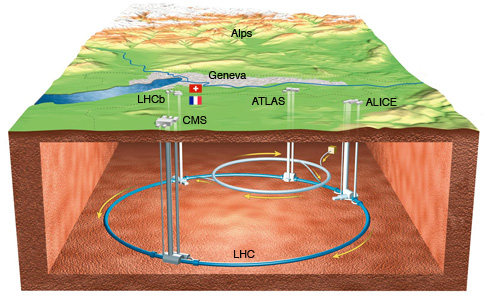
\includegraphics[width=0.8\textwidth]{images/CERNMap.jpg}
%\caption{}
%\label{fig:example2}
\end{center}
\end{figure}

\small{Two very large experiments (Atlas, CMS) with 3500+ people, and two large experiments (Alice, LHCb) with 500+ people}

\end{frame}



\begin{frame}
\frametitle{Plans for upgrading the LHC and Experiment Detectors}

\begin{figure}[htbp]
\begin{center}
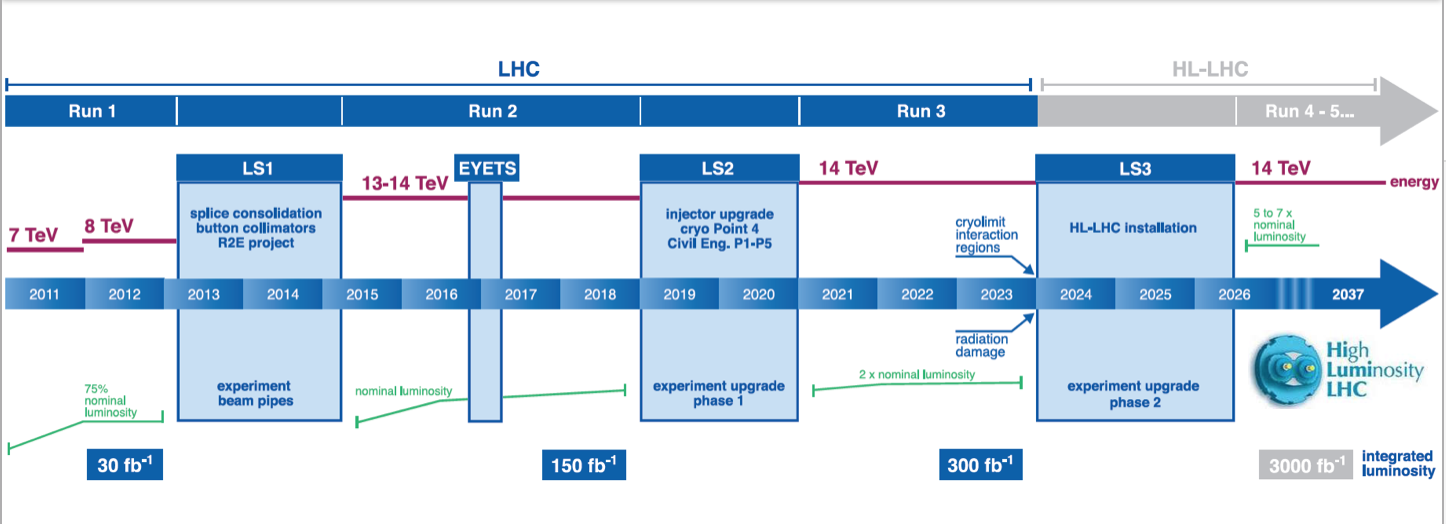
\includegraphics[width=1.0\textwidth]{images/lhc-upgrade-timeline-detail.png}
%\caption{}
%\label{fig:example2}
\end{center}
\end{figure}

\small{The High Luminosity LHC Upgrade is a multi-national, multi-agency 
effort to realize the ultimate physics reach of the LHC. The NSF is
participating and preparations are underway
for a possible ``Major Research Equipment and Facilities Construction'' (MREFC) project to begin in $\sim$2020.}

\end{frame}



\begin{frame}
\frametitle{August 2016 vision of Conceptualization Timeline}

\begin{figure}[htbp]
\begin{center}
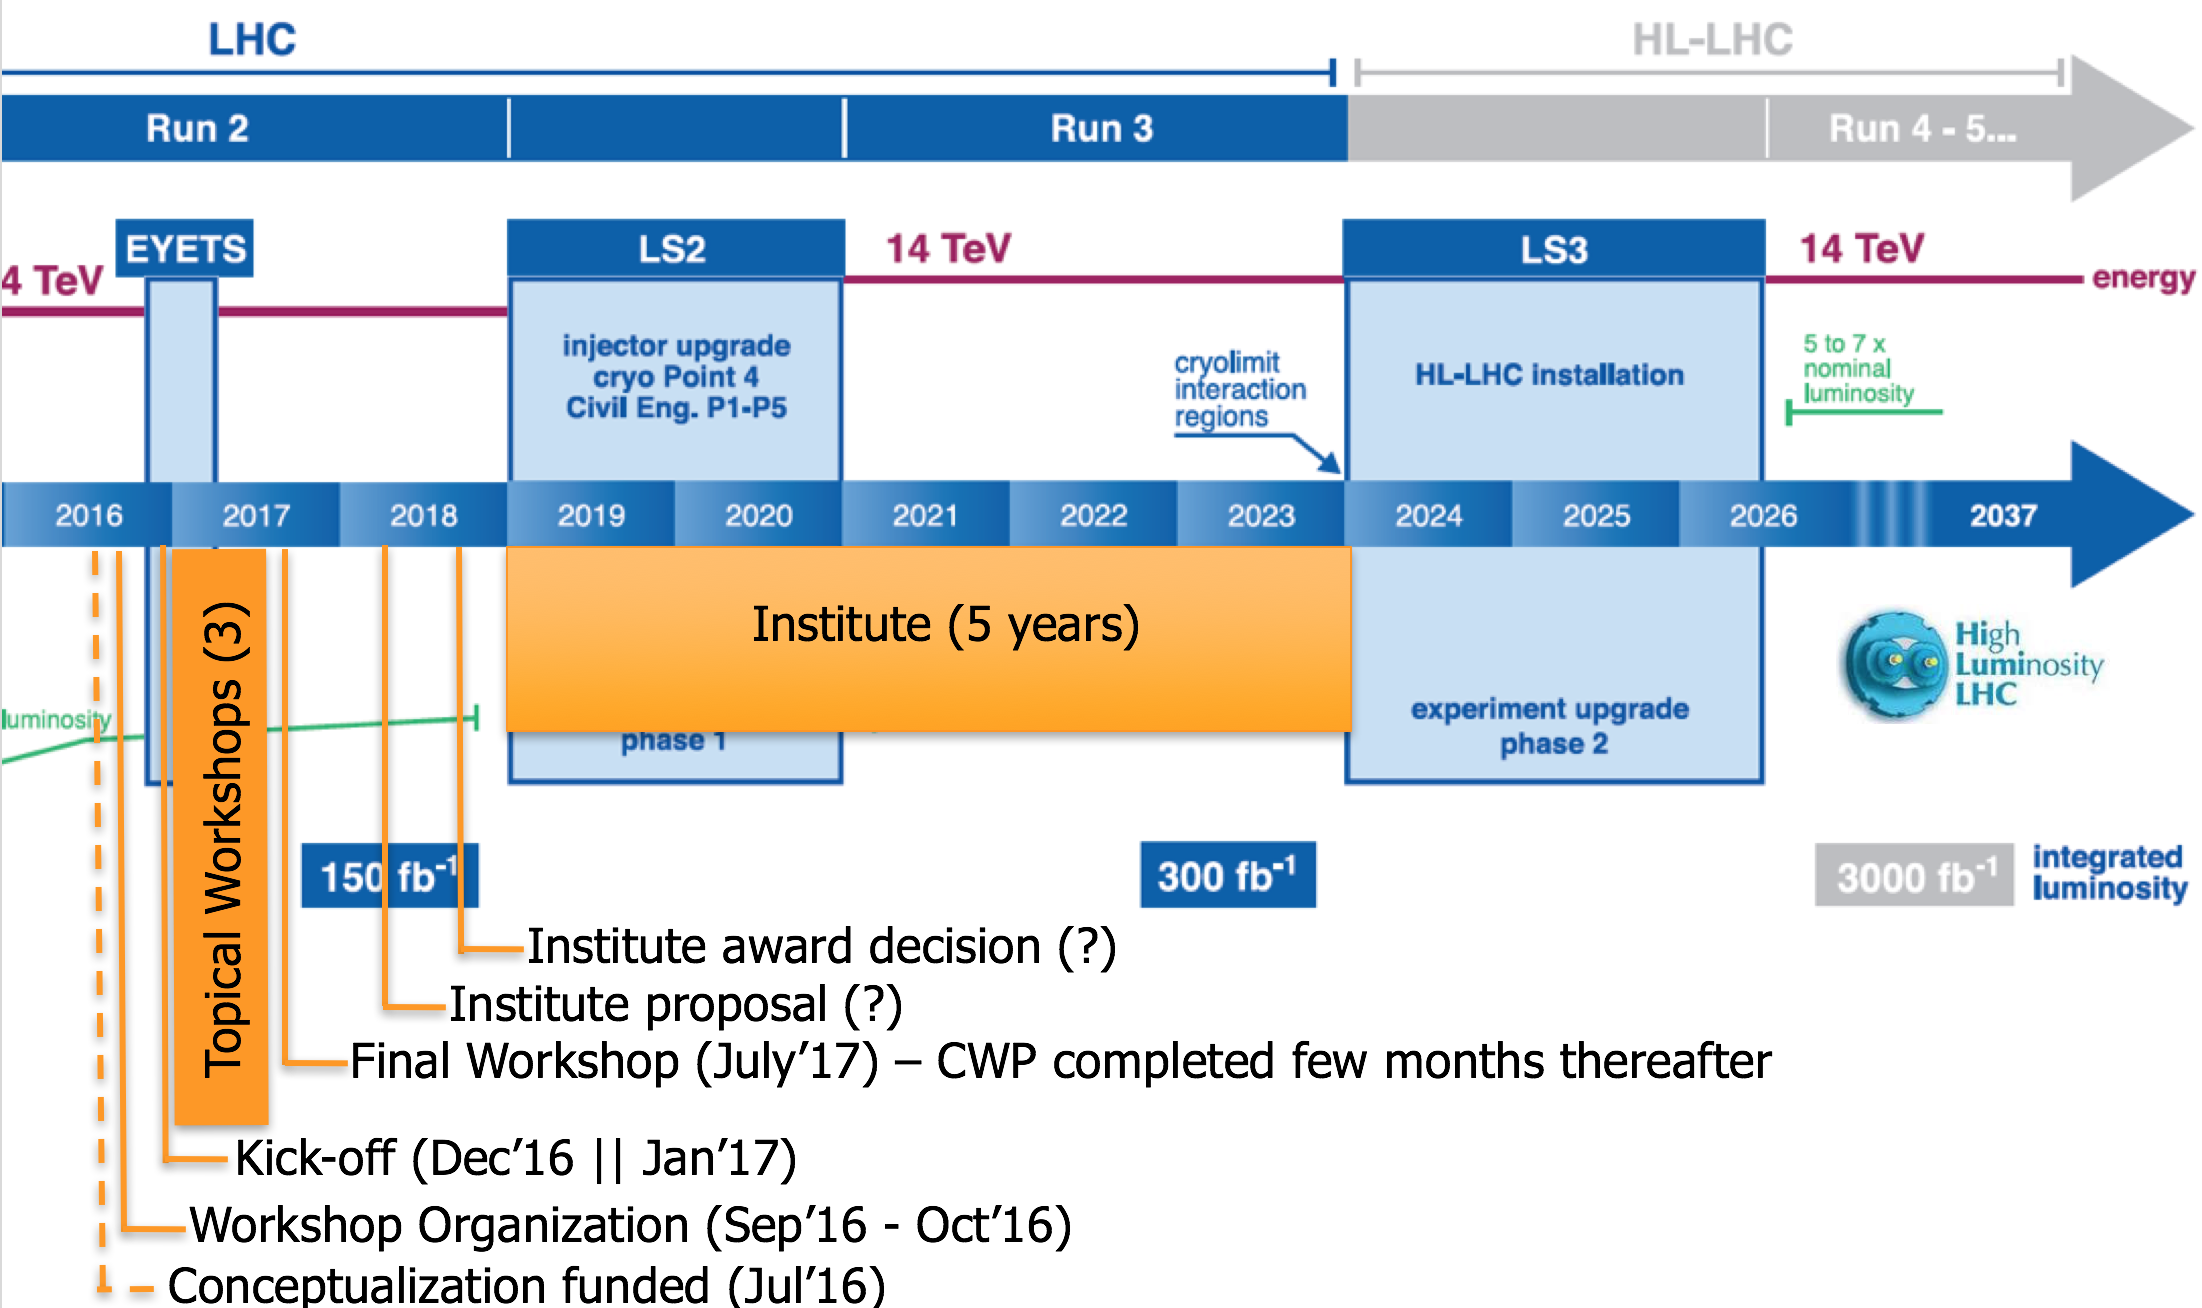
\includegraphics[width=0.9\textwidth]{images/S2I2_timeline.png}
%\caption{}
%\label{fig:example2}
\end{center}
\end{figure}

%\small{Example Text}

\end{frame}



%\begin{frame}
\frametitle{Defining Longer-term Strategy}

\begin{itemize}
\item HL-LHC computing requires a major `software upgrade' and an eventual S2I2 institute for HEP would be a major player in that task
\item Planning for such an ``upgrade'' cannot be done for the US (Universities) in isolation
\item Thus we are intiating a larger community process to produce a Community White Paper (CWP) with an overall consensus strategy and roadmap for software and computing in HEP
  \begin{itemize}
  \item Initiated as WLCG charge to the LHC experiments and HSF as a step towards the LHC experiment TDRs in advance of HL-LHC
  \item The scope should not be restricted only to HL-LHC
  \item Some early software components could be built, tested and used by experiments in LHC Run3
  \end{itemize}
\item Organised by the HEP Software Foundation (HSF) [next slide]
\item Paper to be delivered by Summer 2017
\item The S2I2-HEP Strategic Plan will be derived from this global plan
\end{itemize}

\end{frame}



%\begin{frame}
\frametitle{CWP Charge}

[Switch to pdf file for CWP charge]

\end{frame}



\begin{frame}
\frametitle{HEP Software Ecosystem}

\begin{figure}[htbp]
\begin{center}
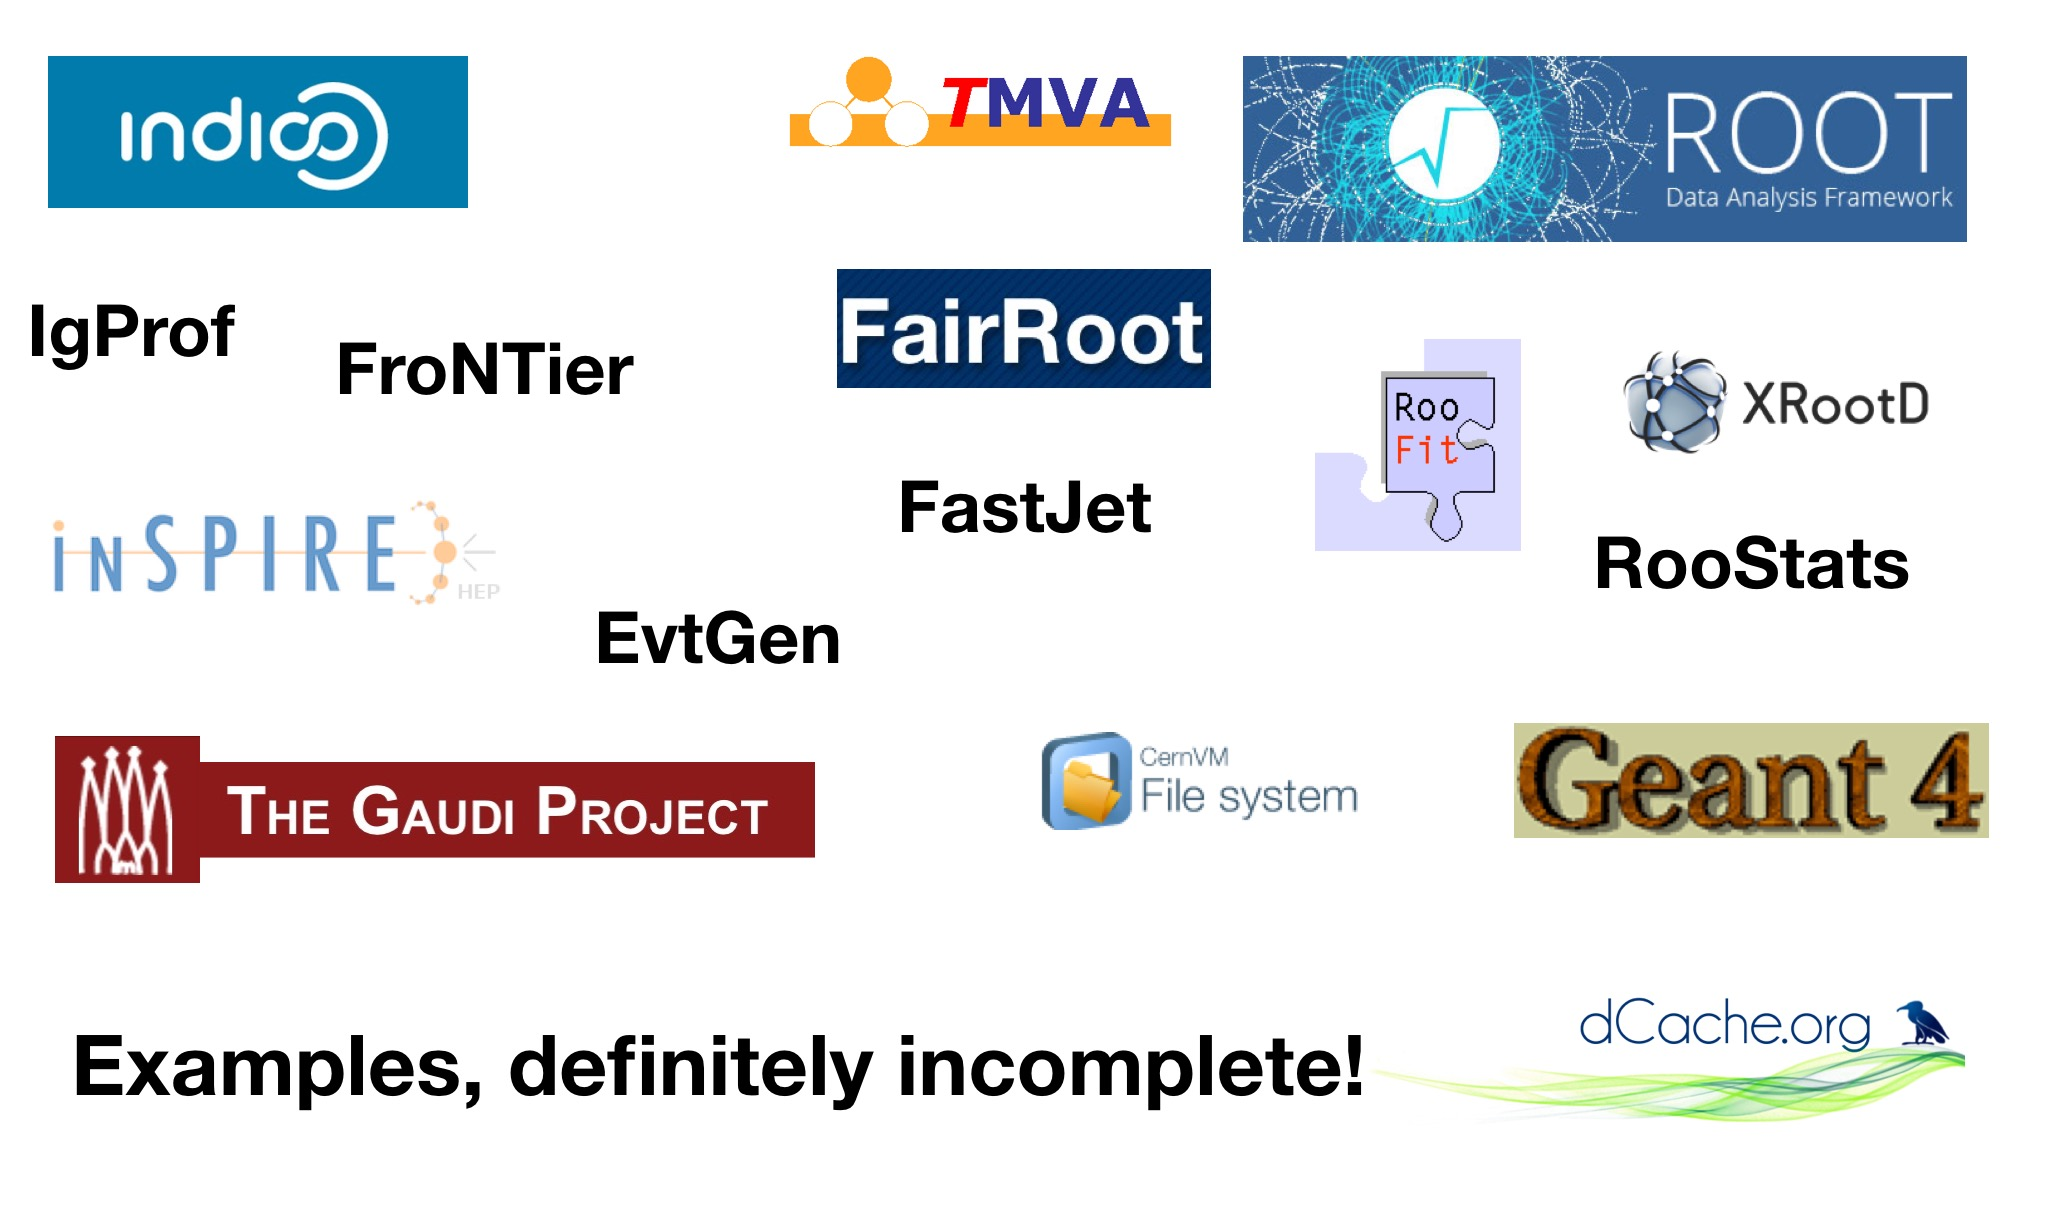
\includegraphics[width=0.9\textwidth]{images/hep-software-ecosystem.jpg}
\end{center}
\end{figure}

{\small Plus 15-20M Source Lines of Code (SLOC) of ``experiment specific'' codes, as well as dependencies on non-HEP scientific software.}
\end{frame}



\begin{frame}
\frametitle{HEP Software Foundation (HSF)}

\begin{columns}[T] % align columns

\begin{column}{.75\textwidth}
The HSF (http://hepsoftwarefoundation.org) was created in early 2015 as a means for organizing our community to address the software challenges of future projects such as the HL-HLC. The HSF has the following objectives: 
\end{column}%

\hfill%

\begin{column}{.20\textwidth}
\begin{figure}[htbp]
\begin{center}

\includegraphics[width=1.0\textwidth]{images/hsf_logo_angled.png}
\end{center}
\end{figure}
\end{column}%

\end{columns}

\vskip 0.1in

\begin{itemize}
\item Catalyze new common projects
\item Promote commonality and collaboration in new developments to make the most of limited resources
\item Provide a framework for attracting effort and support to S\&C common projects (new resources!)
\item Provide a structure to set priorities and goals for the work
\end{itemize}

%An initial set of collaborative activities have begun (see recent HSF workshop 
%at LAL-Orsay). 


\end{frame}



\begin{frame}
\frametitle{(Switch to Webpages)}

S2I2-HEP (workshops) and papers: \url{http://s2i2-hep.org}
\vskip 0.15in
HSF CWP and WG: \url{http://hepsoftwarefoundation.org/activities/cwp.html}
\vskip 0.15in
HSF WG Start:
\url{http://hepsoftwarefoundation.org/cwp/cwp-wg-guidance-sdsc.html}
\end{frame}





%\begin{frame}
\frametitle{Questions - Institute Focus Areas and Priorities}

{\scriptsize


\begin{enumerate}

\item {\bf Impact - Physics:} Will efforts in this area enable new approaches to computing and software that maximize, and could potentially radically extend, the physics reach of the detectors?
\item {\bf Impact - Resources:} Will efforts in this area achieve required improvements in software efficiency, scalability and performance and make use of the advances in CPU, storage and network technologies?
\item {\bf Impact - Sustainability:} Will efforts in this area guarantee the long term sustainability of the software through the lifetime of the HL-LHC?
\item {\bf Interest/Expertise:} Does the U.S.\ university community have a strong interest and expertise in the area?
\item {\bf Leadership:} Are the proposed focus areas complementary to efforts funded by the US-LHC Ops programs, DOE or international entities?
\item {\bf Value:} Is there potential to provide value to more than one LHC experiment and to the wider HEP community?
\item {\bf Research/Innovation:} Are there opportunities for combining research and innovation as part of partnerships between the HEP and Computer Science communities?
%\item Does the area offer opportunities for integration of cutting-edge training and education for our students and postdocs?
\end{enumerate}




}

\end{frame}



\begin{frame}
\frametitle{Impact Criteria (for evaluating each WG topic)}

\begin{enumerate}
\item {\bf Impact - Physics:} Will efforts in this area enable new approaches to computing and software that maximize, and could potentially radically extend, the physics reach of the detectors?
\item {\bf Impact - Resources:} Will efforts in this area achieve required improvements in software efficiency, scalability and performance and make use of the advances in CPU, storage and network technologies?
\item {\bf Impact - Sustainability:} Will efforts in this area guarantee the long term sustainability of the software through the lifetime of the HL-LHC?
\end{enumerate}
\end{frame}



\begin{frame}
\frametitle{On Impact}

``the mighty ships tore across the empty wastes of space and finally dived screaming on to the first planet they came across - which happened to be the Earth - where due to a terrible miscalculation of scale the entire battle fleet was accidentally swallowed by a small dog.'' - Douglas Adams, The Hitchhiker's Guide to the Galaxy

\end{frame}



\begin{frame}
\frametitle{Additional Criteria (for prioritization)}

\begin{enumerate}
\item {\bf Interest/Expertise:} Does the U.S.\ university community have a strong interest and expertise in the area?
\item {\bf Leadership:} Are the proposed focus areas complementary to efforts funded by the US-LHC Ops programs, DOE or international entities?
\item {\bf Value:} Is there potential to provide value to more than one LHC experiment and to the wider HEP community?
\item {\bf Research/Innovation:} Are there opportunities for combining research and innovation as part of partnerships between the HEP and Computer Science communities?
\end{enumerate}

\end{frame}



\begin{frame}
\frametitle{Institute Structure}

\begin{figure}[ht]
\begin{center}
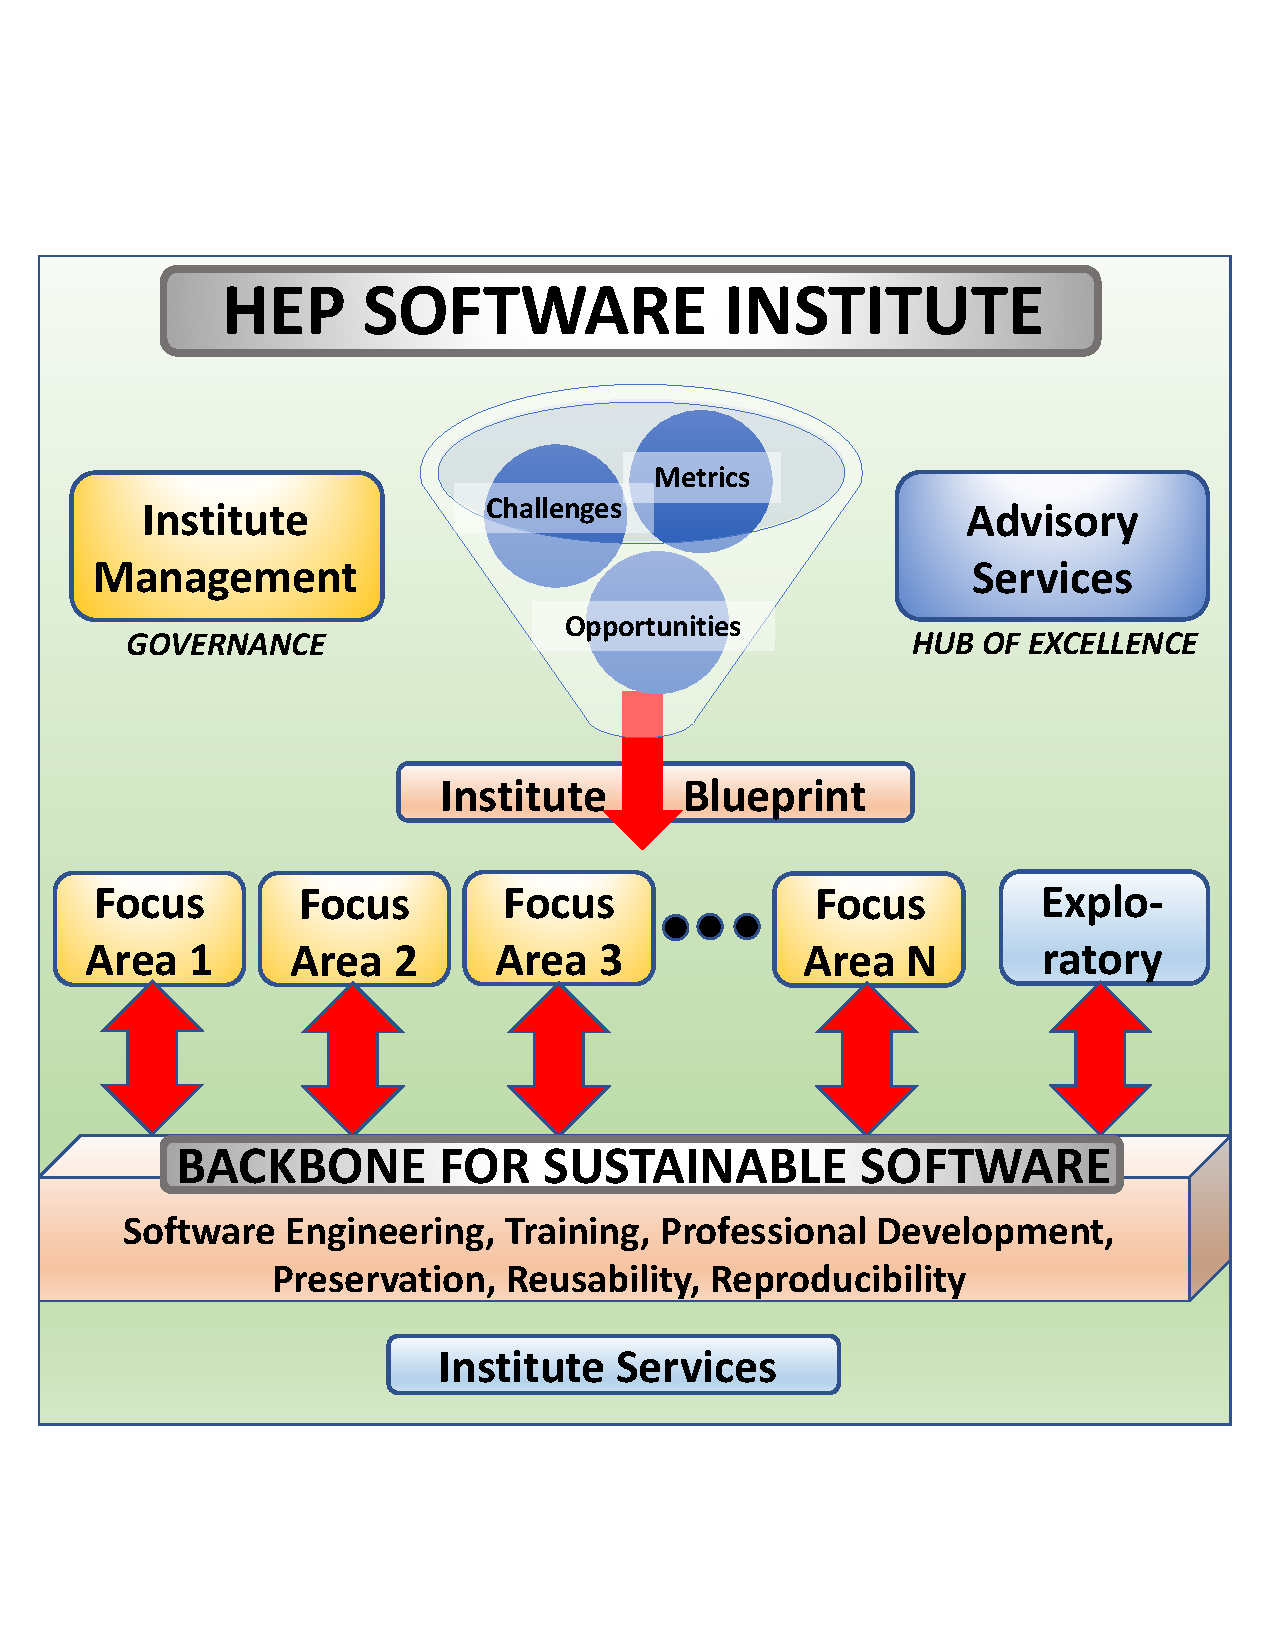
\includegraphics[width=0.5\textwidth]{images/S2I2-HEP_elements_general.pdf}
%\caption{Internal elements of the Institute.}
\label{fig:s2i2_elements}
\end{center}
\end{figure}

\small{4 focus areas (of 10+ Working Groups) were prioritized. (See the Strategic Plan if you care about the details.)}

\end{frame}



\begin{frame}
\frametitle{Blueprint Process}

\begin{figure}[htbp]
\begin{center}
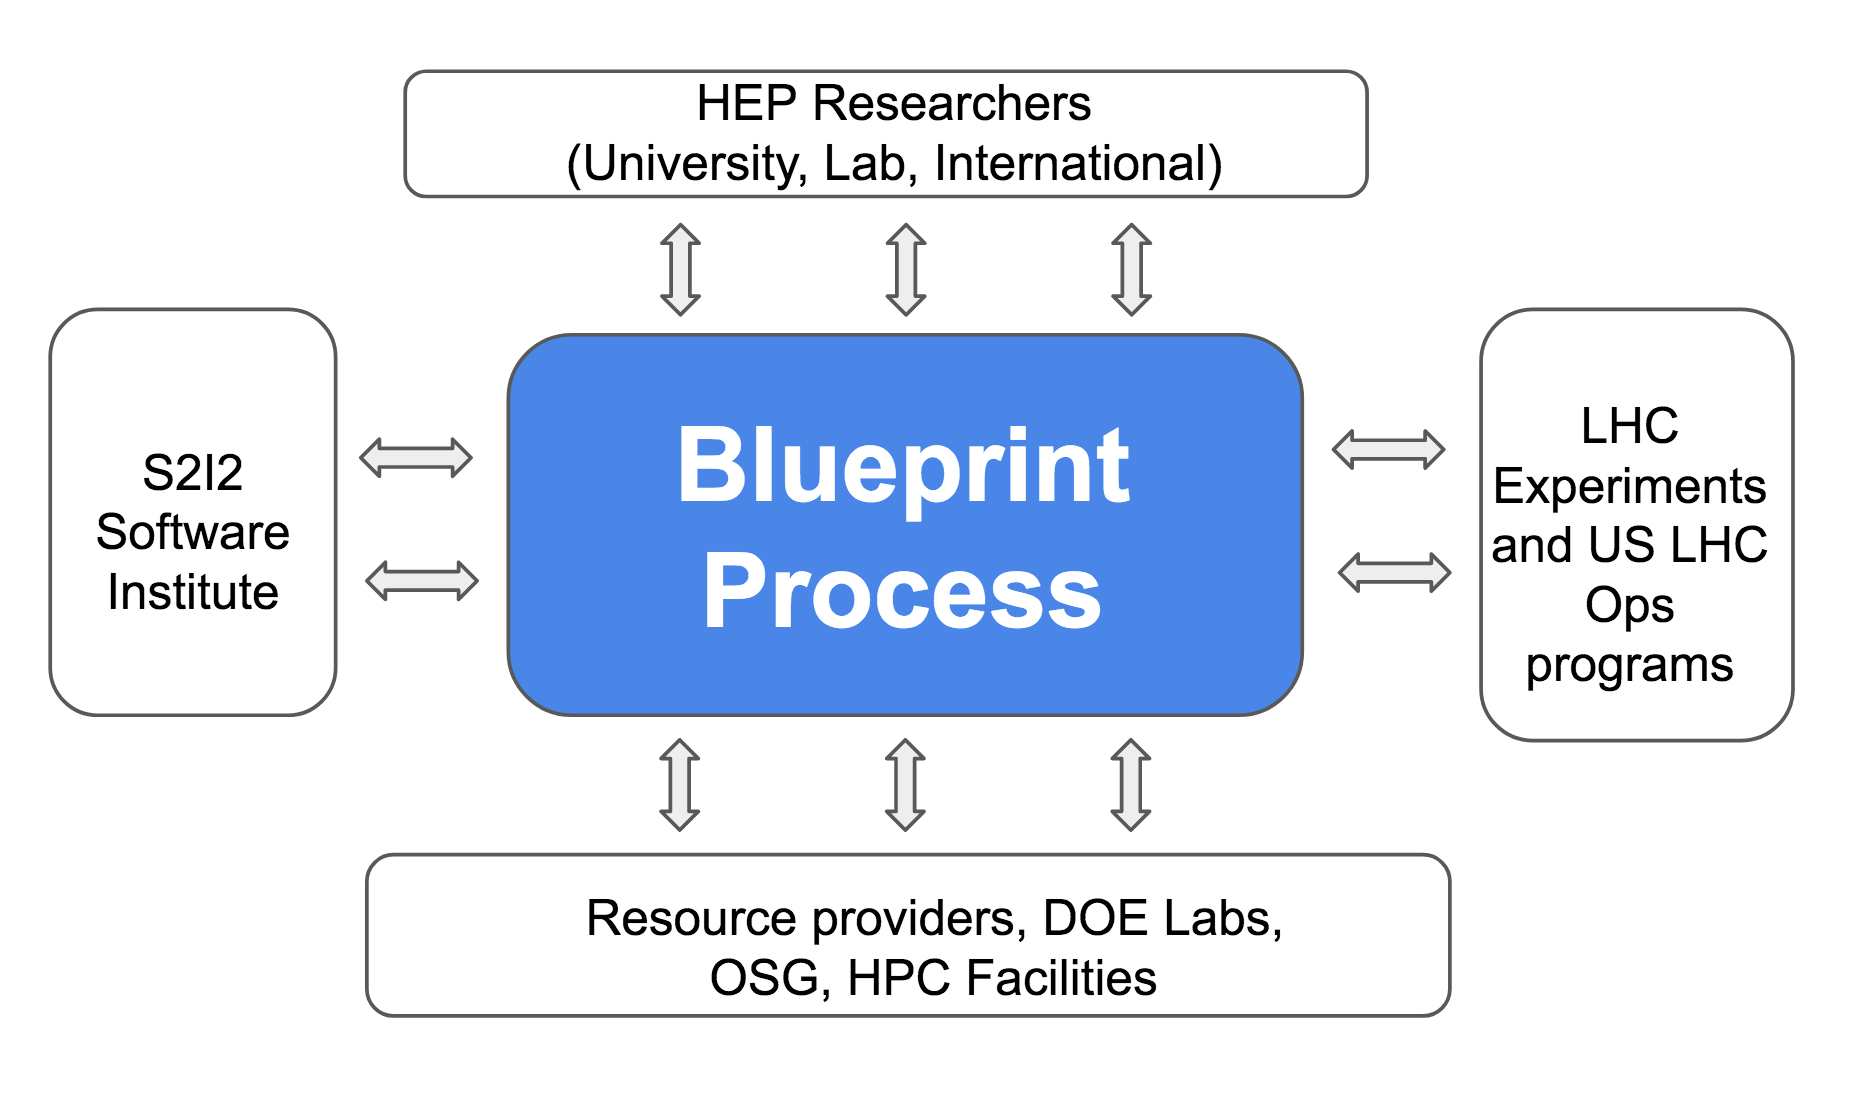
\includegraphics[width=0.8\textwidth]{images/s2i2-global-blueprint-activity.png}
%\caption{}
%\label{fig:example2}
\end{center}
\end{figure}

\small{The Blueprint Process will be a primary means of developing a common vision with the major partners. Blueprint activities will likely happen 3-4 times per year, typically with a focus on a different specific topics each time.}

\end{frame}



\begin{frame}
\frametitle{Extra thoughts}

I made some set of (cryptic) notes as to what we did during our 
conceptualization that helped us. Many already seem integrated into this 
project, but several that aren't (yet) visible (food for thought):
\begin{itemize}
\item Design ``closed loop'' processes for meetings and workshops. Capture the vision. Publicize questions to answer from a meeting in advance and get those answers. Outcome-oriented. Designate people to drive/herd meetings, and to own the process of culling out the answers and agreements/disagreements. Iterate.
\item Clearly separate ``What'' from ``How'' in discussions. Agreeing on what a community wants to do (science driven) is as important as how it does it. The ``Vision'' is not the ``Work Plan''. (Blueprint)
\item Ask questions that encourage more than incrementalism. What if we actually had extra resources? 
\end{itemize}

\end{frame}




\end{document}


